\chapter{Aufbau}



\section{Architektur}

% DrawableGameScreenComponent und GameScreenComponent sind hier wichtige abstrakte Klassen.
% Sie bilden die Schnittstelle zum XNA-Framework. Beide Klassen erben von der XNA-Klasse GameComponent.
% Dabei erbt DrawableGameScreenComponent durch einen zusätzlichen Vererbungsschritt über die Klasse
% DrawableGameComponent von GameComponent. Zudem implementieren die Klassen jeweils noch die Schnittstelle 
% IGameScreenComponent. 

% 2. Satz ->

Die grundlegende Architektur des Spiels basiert auf der Spielkomponenten-Infrastruktur des XNA-Frameworks, die mit Spielzuständen kombiniert wird. Die abstrakten Klassen \class{GameScreenComponent} und \class{DrawableGameScreenComponent} erben von den von XNA bereitgestellten Klassen \xna{GameComponent} und \xna{DrawableGameComponent} und implementieren die Schnittstelle \interface{IGameScreenComponent}. Sie unterscheiden sich von den XNA-Basisklassen dadurch, dass sie immer eine Referenz auf einen bestimmten Spielzustand halten und nur in Kombination mit diesem zu verwenden sind.
\\\\
Die Spielzustände erben von der abstrakten Basisklasse \class{GameScreen} und halten eine Liste von \interface{IGameScreenComponent}-Objekten. Wird ein Spielzustand aktiviert, indem von einem anderen Spielzustand aus zu ihm gewechselt wird oder indem er der Startzustand ist, dann weist er seine Liste von \interface{IGameScreenComponent}-Objekten dem \xna{Components}-Attribut der \class{Game}-Klasse zu, die von der vom XNA-Framework bereitgestellten abstrakten Klasse \xna{Game} erbt. So ist zu jedem Zeitpunkt während der Laufzeit des Spiels ein Spielzustand aktiv, der die aktuelle Liste von Spielkomponenten verwaltet.
\\\\
Die Spielkomponenten, die nicht gezeichnet werden und nur auf Eingaben reagieren, haben nur eine Update()-Methode und erben von \class{GameScreenComponent}. Dies sind vor allem verschiedene Input-Handler, welche Tastatur- und Mauseingaben verarbeiten und beispielsweise die Kameraposition und das Kameratarget ändern oder Spielobjekte bewegen.
\\\\
Spielkomponenten, die neben der Update()-Methode auch eine Draw()-Methode besitzen, erben von \class{DrawableGameScreenComponent}. Dies sind vor allem die Elemente, aus denen die grafische Benutzeroberfläche zusammengesetzt ist, deren abstrakte Basisklasse \class{Widget} darstellt. Dabei gibt es vor allem verschiedene von der abstrakten Klasse \class{MenuItem} erbende Klassen, die Einträge in Menüs darstellen, sowie die Klassen \class{Menu} und \class{VerticalMenu}, die diese in Menüs anordnen. Dargestellt werden diese entweder direkt in den \class{GameScreen}s, etwa in den verschiedenen \class{SettingsScreen}s, oder sie werden vor einer 3D-Szene gerendet und befinden sich in einem \class{Dialog}.
\\\\
Alle Spielobjekte implementieren die Schnittstelle \interface{IGameObject}. Die abstrakte Klasse \class{GameModel} repräsentiert dabei ein Spielobjekt, das aus einem 3D-Modell besteht, und hält zu diesem Zweck eine Referenz auf ein Objekt der Klasse \xna{Model} aus dem XNA-Framework sowie weitere Eigenschaften wie Position, Drehung und Skalierung.

Spielobjekte sind keine Komponenten, sondern werden in einer Spielwelt zusammengefasst, die durch die Klasse \class{World} repräsentiert wird. Die Spielwelt ist ein \class{DrawableGameScreenComponent} und ruft in ihren Update()- und Draw()-Methoden jeweils die dazugehörigen Methoden aller in ihr enthaltenen Spielobjekte auf.
\\\\
Shadereffekte werden durch die abstrakte Klasse \class{RenderEffect} und die von ihr abgeleiteten Klassen gekapselt. Ein \class{RenderEffect} enthält ein Rendertarget vom Typ \xna{RenderTarget2D} als Attribut und implementiert jeweils eine Begin()- und eine End-Methode. In der Methode Begin() wird das aktuell von XNA genutzte Rendertarget auf einem Stack gesichert und das Rendertarget des Effekts wird als aktuelles Rendertarget gesetzt.

Nach dem Aufruf von Begin() werden alle Draw()-Aufrufe von XNA auf dem gesetzten Rendertarget ausgeführt. Es wird also in eine im \xna{RenderTarget2D}-Objekt enthaltene Bitmap gezeichnet. Dabei wird von den Draw()-Methoden der \class{GameModel}s die DrawModel(GameModel)-Methode des \class{RenderEffect}s aufgerufen, der die Modelle mit bestimmten Shadereffekten in die Bitmap zeichnet.

In der End()-Methode wird schließlich das auf dem Stack gesicherte, vorher genutzte Rendertarget wiederhergestellt und das Rendertarget des \class{RenderEffect}s wird, unter Umständen verändert durch Post-Processing-Effekte, auf dieses übergeordnete Rendertarget gezeichnet.


\section{Verwendete Entwurfsmuster}

\subsection{Model View Controller (MVC)}
Unser Entwurf basiert auf dem Entwurfsmuster Model-View-Controller, bei dem die Aufgaben bei einer Anwendung strikt in drei Einheiten aufgeteilt werden. Diese drei Einheiten sind  Datenmodell (Model), Präsentation (View) und Programmsteuerung (Controller).
\newline
\newline
In das Datenmodell werden die Klassen \class{Knot}, \class{Edge} und \class{Circle} eingeteilt, da diese die darzustellenden Daten enthalten und den Controller über Änderungen informieren. Die Präsentation zeigt die Daten in grafischer Form an und informiert die Programmsteuerung über Benutzereingaben. Sie wird von den Klassen \class{PipeModel}, \class{NodeModel} und \class{ArrowModel} repräsentiert.
Der Controller kümmert sich um die Interaktion mit dem Benutzer und entspricht der Klasse \class{KnotRenderer}.

\subsection{Kompositum}
Das Kompositum gehört zu der Kategorie der Varianten-Muster und wird in unserem Entwurf von den Klassen \class{KnotRenderer} und \class{EdgeMovement} in Bezug auf \interface{IGameObject}-Objekte, \interface{IGameScreenComponent} in Bezug auf \class{GameScreen}-Objekte, sowie \class{Menu} und \class{MenuItem} dargestellt.
\newline
\newline
Die Grundidee des Entwurfsmusters Kompositum ist es, in einer abstrakten Klasse sowohl primitive Objekte also auch ihre Behälter zu repräsentieren.
\newline
Dies bedeutet konkret, dass \class{KnotRenderer} und \class{EdgeMovement} sowohl Iteratoren über \interface{IGameObject}-Objekte sind, als auch selbst die Schnittstelle \interface{IGameObject} implementieren und als solche verwendet werden können, indem sie wie einzelne Spielobjekte in der \class{World}-Klasse registriert werden. Die Aufrufe von \interface{IGameObject}-spezifische Methoden wie Draw(), Update() und Intersects(Ray) werden dann auf allen in den Containern enthaltenen \interface{IGameObject}-Objekten ausgeführt.
\newline
\newline
Ein weiteres Beispiel in unserer API stellt die Klasse \class{Widget} dar. Die von \class{Widget} zur Verfügung gestellten Properties und Methoden werden von \class{Menu}, \class{MenuItem}, \class{ColorPicker} und \class{Dialog} implementiert und erweitert.

\subsection{Iterator}
Der Iterator gehört zu der Kategorie der Entkopplungsmuster und wird in unserem Entwurf des Öfteren verwendet, um auf Elemente einer Menge zuzugreifen. Beispielsweise ist ein Objekt der Klasse \class{Knot}, das einen Knoten repräsentiert, ein Iterator über die Kanten (\class{Edge}-Objekte), aus denen der Knoten besteht.


\subsection{Dekorierer}
Der Dekorierer gehört zu der Kategorie der Varianten-Muster und wird von der Klasse \class{ShadowGameObject} dargestellt. 
\class{ShadowGameModel} stellt hierbei einen konkreten Dekorierer dar und erweitert die konkrete Komponente \class{GameModel}.

\subsection{Zustand}
Der Zustand gehört zu der Kategorie der Zustandshandhabungs-Muster und wird von der Klasse \class{GameScreen} repräsentiert. Jeder \class{GameScreen} hat eine eigene grafische Oberfläche und ein eigenes Verhalten.
\class{Knot3Game} stellt den Kontext dar und verwaltet die verschiedenen \class{GameScreen}s. Bei einem Wechsel zwischen verschiedenen \class{GameScreen}s tauscht \class{Knot3Game} die betroffenen \class{GameScreen}s aus.

\section{Klassendiagramm}

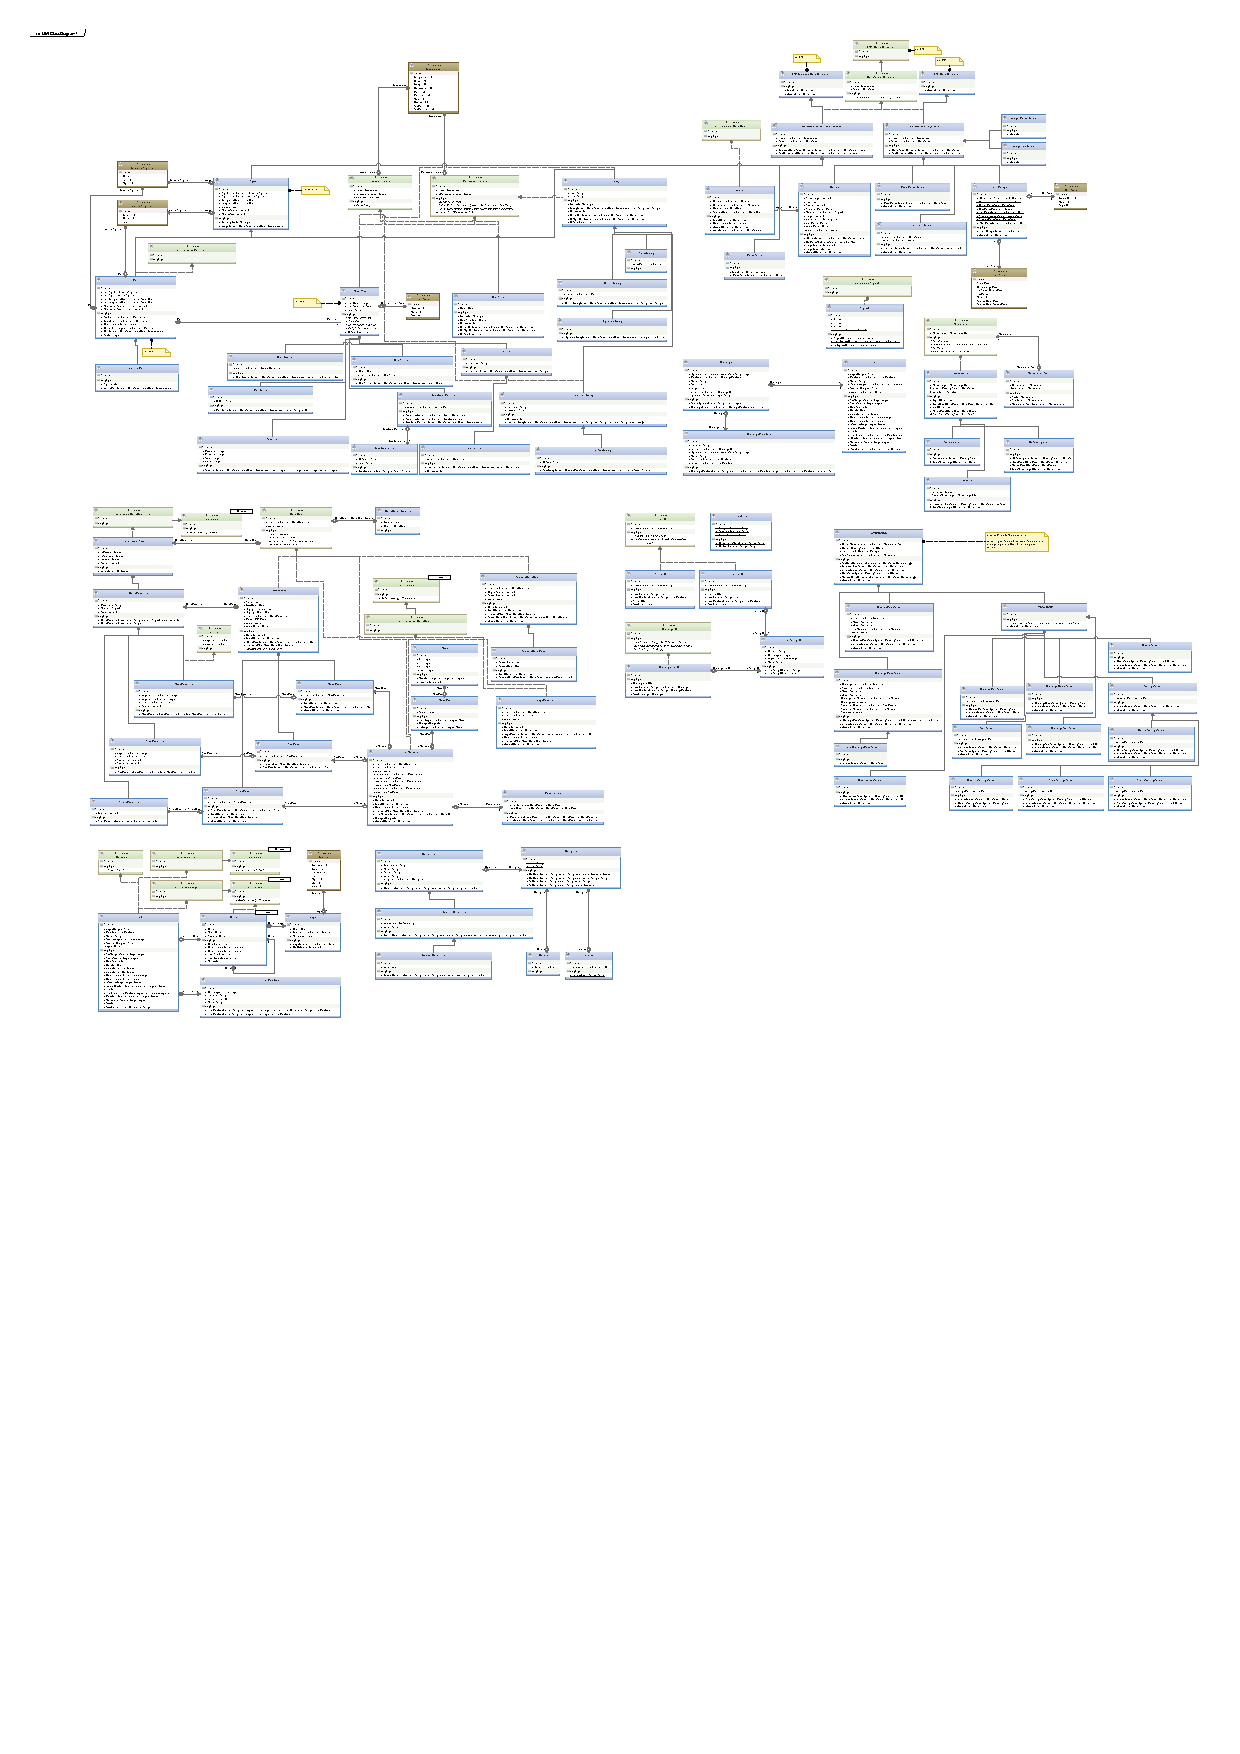
\includegraphics[scale=0.8, trim=0mm 10mm 0mm 0mm]{Klassendiagramm.pdf}